% Intended LaTeX compiler: pdflatex
\documentclass[10pt,a4paper,UTF8]{article}
\usepackage{zclorg}
\author{张朝龙}
\date{}
\title{练习:基}
\hypersetup{
 pdfauthor={张朝龙},
 pdftitle={练习:基},
 pdfkeywords={},
 pdfsubject={},
 pdfcreator={Emacs 25.0.50.1 (Org mode 9.0.5)}, 
 pdflang={English}}
\begin{document}

\maketitle
\tableofcontents
\titlepic{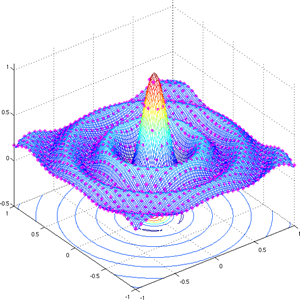
\includegraphics[scale=0.25]{../../img/sinc.PNG}}


\section*{2.b.1}
\label{sec:orgeb37aa7}


\begin{problem}
找出只含一个基的所有向量空间。
\end{problem}

\begin{answer}
答案很简单只有\(\{0\}\)是含有一个基的向量空间。因为若\(v\)是向量空间的一个基,则显然有\(\lambda v,\lambda \neq 0\)也是该向量空间的一个基。
\end{answer}
\section*{2.b.3}
\label{sec:org1222308}


\begin{problem}
设\(U\)是\(\mathbf{R}^{5}\)的子空间,\(U=\{(x_{1},x_{2},x_{3},x_{4},x_{5})\in \mathbf{R}^{5}:x_{1}=3x_{2},x_{3}=7x_{4}\}\)求\(U\)的一个基
\end{problem}

\begin{answer}
设\(x_{2},x_{4},x^{5}\)是自由变量。我们可以采取很简单的做法,当某个元素为1的时候,其他两个为0.显然有
\begin{eqnarray*}
&&(3,1,0,0,0)\\
&&(0,0,7,1,0)\\
&&(0,0,0,0,1)
\end{eqnarray*}
\end{answer}

\begin{problem}
将上一步的基扩充成\(\mathbf{R}^{5}\)的基。我们知道
\begin{eqnarray*}
&&(3,1,0,0,0)\\
&&(0,0,7,1,0)\\
&&(0,0,0,0,1)
\end{eqnarray*}
是线性无关组,且向量个数为3,我们需要再扩充两个向量才能构成\(\mathbf{R}^{5}\)的基.可以扩充:
\begin{eqnarray*}
&&(1,0,0,0,0)\\
&&(0,0,1,0,0)
\end{eqnarray*}
这两个线性无关向量。
\end{problem}

\begin{problem}
找出\(\mathbf{R}^{5}\)的一个子空间\(W\)使得\(\mathbf{R}^{5} = U\oplus W\)
\end{problem}

\begin{answer}
首先令\(U=\{(x_{1},x_{2},x_{3},x_{4},x_{5})\in \mathbf{R}^{5}:x_{1}=3x_{2},x_{3}=7x_{4}\}\),我们知道这个空间的一个基是:
\begin{eqnarray*}
&&(3,1,0,0,0)\\
&&(0,0,7,1,0)\\
&&(0,0,0,0,1)
\end{eqnarray*}

另外根据第二步,我们扩充了:
\begin{eqnarray*}
&&(1,0,0,0,0)\\
&&(0,0,1,0,0)
\end{eqnarray*}
这两个向量,从而构成了\(\mathbf{R}^{5}\)的一个基。所以可以得知由这两个向量张成的子空间构成了\(W\),使得\(V = U\oplus W\)
显然我们可以把\(W\)写成:
\(W=\{(x_{1},x_{2},x_{3},x_{4},x_{5})\in \mathbf{R}^{5}:x_{2}=x_{3}=x_{4}=x_{5}=0 \quad or\quad x_{1}=x_{2}=x_{4}=x_{5}=0   \}\)
\end{answer}
\section*{2.b.4}
\label{sec:orgabae076}


\begin{problem}
设\(U\)是\(\mathbf{C}^{5}\) 的子空间,\(U=\{(z_{1},z_{2},z_{3},z_{4},z_{5})\in \mathbf{C}^{5}:6z_{1}=z_{2},z_{3} + 2z_{4} + 3z_{5} =0\}\),求\(U\)的一个基。
\end{problem}

\begin{answer}
根据2.b.3我们有:
\begin{eqnarray*}
&&(6,1,0,0,0)\\
&&(0,0,-2,1,0)\\
&&(0,0,-3,0,1)
\end{eqnarray*}
\end{answer}

\begin{problem}
将上题的基扩展成\(\mathbf{C}^{5}\)的基
\end{problem}

\begin{answer}
我们只需要再扩展两个向量,和之前的三个向量构成线性无关组即可。
\begin{eqnarray*}
&&(1,0,0,0,0)\\
&&(0,0,1,0,0)
\end{eqnarray*}
\end{answer}

\begin{problem}
找出\(\mathbf{C}^{5}\)的一个字空间\(W\)使得\(\mathbf{C}^{5} = U \oplus W\)
\end{problem}

\begin{answer}
只要把后来扩展的线性无关组张成的空间作为\(W\)即可:
\(W= span((1,0,0,0,0),(0,0,0,1))\)
\end{answer}

\section*{2.b.5}
\label{sec:orgdc9b632}


\begin{problem}
证明或反驳:\(\mathcal{P}_{3}(F)\)有一个基\(p_{0},p_{1},p_{2},p_{3}\)使得多项式\(p_{0},p_{1},p_{2},p_{3}\)的次数都不等于2.
\end{problem}

\begin{answer}
我们知道\(1,x,x^{2},x^{3}\)构成了\(\mathcal{P}_{3}(\mathbf{F})\)的一个基。对于另外一组向量\(1,x,x^{3}-x^{2},x^{3}+x^{2}\),可以得到对于任何\(a_{i}\in \mathbf{F}\),有
\begin{equation}
\label{eq:1}
0=a_{0} + a_{1} x + a_{2}(x^{3}-x^{2}) + a_{3}(x_{3}+x^{2})
\end{equation}
整理后:
\begin{equation}
\label{eq:2}
0=a_{0} + a_{1} x + (a_{3} - a_{2})x^{2} + (a_{3}+a_{2})x^{3}
\end{equation}

因为\(1,x,x^{2},x^{3}\)线性无关,则有\(a_{0},\ldots ,a_{3}\)都是零。所以有\(1,x,x^{3}-x^{2},x^{3}+x^{2}\)是线性无关的。又因为\(\mathcal{P}_{3}(\mathbf{F})\)是有限维的。且线性无关组\(1,x,x^{3}-x^{2},x^{3}+x^{2}\)是线性无关的,长度为5,所以\(1,x,x^{3}-x^{2},x^{3}+x^{2}\)是\(\mathcal{P}_{3}(F)\)的一个基。
\end{answer}
\section*{2.b.6}
\label{sec:org2326aa7}


\begin{problem}
设\(v_{1},v_{2},v_{3},v_{4}\)是\(V\)的基,证明\(v_{1}+v_{2},v_{2}+v_{3},v_{3}+v_{4},v_{4}\)也是\(V\)的基。
\end{problem}

\begin{answer}
首先这两个向量组的长度都是4。我们只需要证明\(v_{1}+v_{2},v_{2}+v_{3},v_{3}+v_{4},v_{4}\)也是线性无关的即可。

设有\(a_{i}\in \mathbf{F}\),使得:
\begin{equation}
\label{eq:3}
0= a_{1}(v_{1} +v_{2}) + a_{2}(v_{2} + v_{3}) + a_{3}(v_{3}+v_{4}) + a_{4}v_{4}
\end{equation}

则有:
\begin{equation}
\label{eq:4}
0 = a_{1}v_{1} + (a_{1}+a_{2})v_{2} + (a_{2}+a_{3})v_{3} + (a_{3} + a_{4})v_{4}
\end{equation}

因为\(v_{1},v_{2},v_{3},v_{4}\)是\(V\)的基,所以线性无关,所以\(a_{i}=0,i=1,\ldots ,4\)

所以\(v_{1}+v_{2},v_{2}+v_{3},v_{3}+v_{4},v_{4}\)也线性无关。
\end{answer}

\section*{2.b.7}
\label{sec:org2ab534f}


\begin{problem}
证明或反驳:若\(v_{1},v_{2},v_{3},v_{4}\)是\(V\)的基,且\(U\)是\(V\)的子空间。使得\(v_{1},v_{2}\in U\),\(v_{3},v_{4}\notin U\),则\(v_{1},v_{2}\)是\(U\)的基。
\end{problem}

\begin{answer}
乍看这个命题是真的。\(V\)可以划分为\(U\oplus W\),但是这里没有说\(U,W\)的张成组分别有多少个线性无关向量,可能\(U,W\)的张成组都有两个线性无关向量,也可能\(U\)的张成组有三个线性无关向量,而\(W\)的张成组有1个线性无关向量。比如
\begin{eqnarray*}
v_{1}&=&(1,0,0,0) \\
v_{2}&=&(0,1,0,0) \\
v_{3}&=&(0,0,1,1) \\
v_{4}&=&(0,0,0,1) 
\end{eqnarray*}
假设\(U=\{(x,y,z,0)\in \mathbf{R}^{4}:x,y,z\in \mathbf{R}\}\),满足\(v_{1}\in U,v_{2}\in U\),\(v_{3}\notin U,v_{4}\notin U\),但是\(v_{1},v_{2}\)不是\(U\)的基。

我最开始的思考漏掉了什么?

漏掉了\(U\)的基有三个向量无关组的情形。
\end{answer}
\section*{2.b.8}
\label{sec:orgd4a54fa}


\begin{problem}
设\(U,W\)是\(V\)的子空间,使得\(V=U\oplus W\),并设\(u_{1},\ldots ,u_{m}\)是\(U\)的基,\(w_{1},\ldots ,w_{n}\)是\(W\)的基,证明\(u_{1},\ldots ,u_{m},w_{1},\ldots ,w_{n}\)是\(V\)的基。
\end{problem}

\begin{answer}
证明因为\(V=U\oplus W\),对于\(V\)总的任意一个向量\(v\)都有唯一的一个\(u\in U,w\in W\)使得\(v = u+w,u\in U, w\in W\)。 而对于\(u\in U\)有唯一的一组\(a_{i}\in \mathbf{F}\)使得:
\begin{equation}
\label{eq:5}
u = a_{1}u_{1}+\ldots a_{m}u_{m}
\end{equation}
同理对于\(w\)有:
\begin{equation}
\label{eq:6}
w = b_{1}w_{1}+\ldots b_{m}w_{m}
\end{equation}
所以有:
\begin{equation}
\label{eq:7}
v = a_{1}u_{1}+\ldots a_{m}u_{m} + b_{1}w_{1}+\ldots b_{n}w_{n}
\end{equation}
且这种表示方式是唯一的,所以\(u_{1},\ldots ,u_{m},w_{1},\ldots ,w_{n}\)张成\(V\),表示方式是唯一的。

另外假设存在\(a_{i}\in \mathbf{F},b_{i} \in \mathbf{F}\),使得:
\begin{equation}
\label{eq:8}
 a_{1}u_{1}+\ldots a_{m}u_{m} + b_{1}w_{1}+\ldots b_{n}w_{n} = 0
\end{equation}
则有:
\begin{equation}
\label{eq:9}
 a_{1}u_{1}+\ldots a_{m}u_{m} = -( b_{1}w_{1}+\ldots b_{n}w_{n}) \in U\cap W
\end{equation}

又因为\(V=U\oplus W\),则\(\{0\} = U\oplus W\),则有:
\begin{eqnarray*}
 a_{1}u_{1}+\ldots a_{m}u_{m} &=&0\\
b_{1}w_{1}+\ldots b_{n}w_{n} &=&0
\end{eqnarray*}
又因为\(u_{1},\ldots ,u_{m}\)是\(U\)的基,\(w_{1},\ldots ,w_{n}\)是\(W\)的基,则有\(a_{i}=0,b_{i}=0\),所以\(u_{1},\ldots ,u_{m},w_{1},\ldots ,w_{n}\) 是线性独立的。

综上\(u_{1},\ldots ,u_{m},w_{1},\ldots ,w_{n}\)是\(V\)的基。

证明任何向量组是空间的基要分两步:1)证明张成,2)证明线性无关。
\end{answer}
\end{document}
